\question \textbf{N-grams}
  
N-grams are n-letter words that can be used for database search methods. Create a table of 2-grams for q: ATGCAT.

\vspace{0.1 in}

\begin{parts}

%% (a)
  \part List all 2-grams of q.

\begin{solution}[0.5 in]
\begin{verbatim}
  AT, TG, GC, CA, AT
\end{verbatim}
\end{solution}

%% (b)
\part Fill the table with the 2-grams and the corresponding indices of q.

\begin{figure}[H]
      \centering
      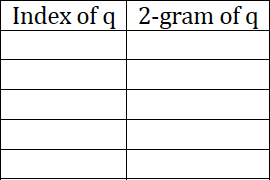
\includegraphics[width=0.25 \textwidth]{fig05/n-gram.png}
\end{figure}

\end{parts}

